\def\year{2022}\relax
%File: formatting-instructions-latex-2022.tex
%release 2022.1
\documentclass[letterpaper]{article} % DO NOT CHANGE THIS
\usepackage{amsmath}
\usepackage{amssymb}
\usepackage{amsthm}
\usepackage[table]{xcolor}
\usepackage{makecell}
\usepackage{floatrow}
 \floatsetup[table]{capposition=bottom}
\usepackage{color}
% \floatsetup[table]{capposition=top}
\newfloatcommand{capbtabbox}{table}[][\FBwidth]
\usepackage{aaai22}  % DO NOT CHANGE THIS
\usepackage{times}  % DO NOT CHANGE THIS
\usepackage{helvet}  % DO NOT CHANGE THIS
\usepackage{courier}  % DO NOT CHANGE THIS
\usepackage[hyphens]{url}  % DO NOT CHANGE THIS
\usepackage{graphicx} % DO NOT CHANGE THIS
\urlstyle{rm} % DO NOT CHANGE THIS
\def\UrlFont{\rm}  % DO NOT CHANGE THIS
\usepackage{natbib}  % DO NOT CHANGE THIS AND DO NOT ADD ANY OPTIONS TO IT
\usepackage{caption} % DO NOT CHANGE THIS AND DO NOT ADD ANY OPTIONS TO IT
\DeclareCaptionStyle{ruled}{labelfont=normalfont,labelsep=colon,strut=off} % DO NOT CHANGE THIS
\frenchspacing  % DO NOT CHANGE THIS
\setlength{\pdfpagewidth}{8.5in}  % DO NOT CHANGE THIS
\setlength{\pdfpageheight}{11in}  % DO NOT CHANGE THIS
%
% These are recommended to typeset algorithms but not required. See the subsubsection on algorithms. Remove them if you don't have algorithms in your paper.
\usepackage{algorithm}
\usepackage{algorithmic}

%
% These are are recommended to typeset listings but not required. See the subsubsection on listing. Remove this block if you don't have listings in your paper.
\usepackage{newfloat}
\usepackage{listings}
\lstset{%
	basicstyle={\footnotesize\ttfamily},% footnotesize acceptable for monospace
	numbers=left,numberstyle=\footnotesize,xleftmargin=2em,% show line numbers, remove this entire line if you don't want the numbers.
	aboveskip=0pt,belowskip=0pt,%
	showstringspaces=false,tabsize=2,breaklines=true}
\floatstyle{ruled}
\newfloat{listing}{tb}{lst}{}
\floatname{listing}{Listing}
%
%\nocopyright
%
% PDF Info Is REQUIRED.
% For /Title, write your title in Mixed Case.
% Don't use accents or commands. Retain the parentheses.
% For /Author, add all authors within the parentheses,
% separated by commas. No accents, special characters
% or commands are allowed.
% Keep the /TemplateVersion tag as is
\pdfinfo{
/Title (AAAI Press Formatting Instructions for Authors Using LaTeX -- A Guide)
/Author (AAAI Press Staff, Pater Patel Schneider, Sunil Issar, J. Scott Penberthy, George Ferguson, Hans Guesgen, Francisco Cruz, Marc Pujol-Gonzalez)
/TemplateVersion (2022.1)
}

% DISALLOWED PACKAGES
% \usepackage{authblk} -- This package is specifically forbidden
% \usepackage{balance} -- This package is specifically forbidden
% \usepackage{color (if used in text)
% \usepackage{CJK} -- This package is specifically forbidden
% \usepackage{float} -- This package is specifically forbidden
% \usepackage{flushend} -- This package is specifically forbidden
% \usepackage{fontenc} -- This package is specifically forbidden
% \usepackage{fullpage} -- This package is specifically forbidden
% \usepackage{geometry} -- This package is specifically forbidden
% \usepackage{grffile} -- This package is specifically forbidden
% \usepackage{hyperref} -- This package is specifically forbidden
% \usepackage{navigator} -- This package is specifically forbidden
% (or any other package that embeds links such as navigator or hyperref)
% \indentfirst} -- This package is specifically forbidden
% \layout} -- This package is specifically forbidden
% \multicol} -- This package is specifically forbidden
% \nameref} -- This package is specifically forbidden
% \usepackage{savetrees} -- This package is specifically forbidden
% \usepackage{setspace} -- This package is specifically forbidden
% \usepackage{stfloats} -- This package is specifically forbidden
% \usepackage{tabu} -- This package is specifically forbidden
% \usepackage{titlesec} -- This package is specifically forbidden
% \usepackage{tocbibind} -- This package is specifically forbidden
% \usepackage{ulem} -- This package is specifically forbidden
% \usepackage{wrapfig} -- This package is specifically forbidden
% DISALLOWED COMMANDS
% \nocopyright -- Your paper will not be published if you use this command
% \addtolength -- This command may not be used
% \balance -- This command may not be used
% \baselinestretch -- Your paper will not be published if you use this command
% \clearpage -- No page breaks of any kind may be used for the final version of your paper
% \columnsep -- This command may not be used
% \newpage -- No page breaks of any kind may be used for the final version of your paper
% \pagebreak -- No page breaks of any kind may be used for the final version of your paperr
% \pagestyle -- This command may not be used
% \tiny -- This is not an acceptable font size.
% \vspace{- -- No negative value may be used in proximity of a caption, figure, table, section, subsection, subsubsection, or reference
% \vskip{- -- No negative value may be used to alter spacing above or below a caption, figure, table, section, subsection, subsubsection, or reference

\setcounter{secnumdepth}{0} %May be changed to 1 or 2 if section numbers are desired.

% The file aaai22.sty is the style file for AAAI Press
% proceedings, working notes, and technical reports.
%

% Title

% Your title must be in mixed case, not sentence case.
% That means all verbs (including short verbs like be, is, using,and go),
% nouns, adverbs, adjectives should be capitalized, including both words in hyphenated terms, while
% articles, conjunctions, and prepositions are lower case unless they
% directly follow a colon or long dash
\title{Dual Energy-Flow Enhanced Graph Neural Network\\ for Visual Question Answering}
% \author{
%     %Authors
%     % All authors must be in the same font size and format.
%     Written by AAAI Press Staff\textsuperscript{\rm 1}\thanks{With help from the AAAI Publications Committee.}\\
%     AAAI Style Contributions by Pater Patel Schneider,
%     Sunil Issar,\\
%     J. Scott Penberthy,
%     George Ferguson,
%     Hans Guesgen,
%     Francisco Cruz\equalcontrib,
%     Marc Pujol-Gonzalez\equalcontrib
% }
% \affiliations{
%     %Afiliations
%     \textsuperscript{\rm 1}Association for the Advancement of Artificial Intelligence\\
%     % If you have multiple authors and multiple affiliations
%     % use superscripts in text and roman font to identify them.
%     % For example,

%     % Sunil Issar, \textsuperscript{\rm 2}
%     % J. Scott Penberthy, \textsuperscript{\rm 3}
%     % George Ferguson,\textsuperscript{\rm 4}
%     % Hans Guesgen, \textsuperscript{\rm 5}.
%     % Note that the comma should be placed BEFORE the superscript for optimum readability

%     2275 East Bayshore Road, Suite 160\\
%     Palo Alto, California 94303\\
%     % email address must be in roman text type, not monospace or sans serif
%     publications22@aaai.org
% %
% % See more examples next
% }

% %Example, Single Author, ->> remove \iffalse,\fi and place them surrounding AAAI title to use it
% \iffalse
% \title{My Publication Title --- Single Author}
% \author {
%     Author Name
% }
% \affiliations{
%     Affiliation\\
%     Affiliation Line 2\\
%     name@example.com
% }
% \fi

% \iffalse
% %Example, Multiple Authors, ->> remove \iffalse,\fi and place them surrounding AAAI title to use it
% \title{My Publication Title --- Multiple Authors}
% \author {
%     % Authors
%     First Author Name,\textsuperscript{\rm 1}
%     Second Author Name, \textsuperscript{\rm 2}
%     Third Author Name \textsuperscript{\rm 1}
% }
% \affiliations {
%     % Affiliations
%     \textsuperscript{\rm 1} Affiliation 1\\
%     \textsuperscript{\rm 2} Affiliation 2\\
%     firstAuthor@affiliation1.com, secondAuthor@affilation2.com, thirdAuthor@affiliation1.com
% }
% \fi


% REMOVE THIS: bibentry
% This is only needed to show inline citations in the guidelines document. You should not need it and can safely delete it.
\usepackage{bibentry}
% END REMOVE bibentry

\begin{document}

\maketitle

\begin{abstract}
% Scene Graphs (SG), as a structural abstraction of natural images, contain massive detailed information. 
% Modeling visual reasoning through SG can significantly improve the ability and strengthen the interpretability of reasoning. 
% However, neither can existing models \emph{jointly} exploit objects, relations, and attributes information in SG, nor can they balance the importance of objects and relations. 
% In this paper, we introduce a novel Dual Energy-Flow Enhanced Graph Neural Network (DE-GNN), which learns a comprehensive representation by encoding full-scale scene graphs information from objects, attributes, and relations.
% Specifically, two types of SG structures are employed in the encoder: 
% (i) \textit{Object-significant graphs} which absorb attribute and relation information into nodes' representations. 
% (ii) \textit{Relation-significant graphs} which intensify the model's perception of relation features. 
% In addition, we design an \textit{energy-flow mechanism} to enhance the information transfer from edges and adjacent nodes to the updating nodes. 
% We conduct extensive experiments on public GQA and Visual Genome datasets and achieve new state-of-the-art performances highlighting the benefits of our method. 

Scene graph, as a structural abstraction of natural images, contains massive, detailed information. Modeling visual reasoning through scene graphs can significantly improve the ability and strengthen the interpretability of reasoning. However, neither does one of these models \emph{jointly} exploit objects, relations, and attributes information in scene graph, nor does one of them balance the importance of objects and relations. In this paper, we introduce a novel Dual Energy-Flow Enhanced Graph Neural Network (DE-GNN), which learns a comprehensive representation by encoding full-scale scene graph information from objects, attributes, and relations. Specifically, two types of scene graph structures are employed in the encoder: (i) \textit{Object-significant graph} which embeds attribute and relation information into node representations. (ii) \textit{Relation-significant graph} which intensifies the model perception of relation features. In addition, we design an \textit{energy-flow mechanism} to enhance the information transferred from edges and adjacent nodes to updating nodes.
We conduct extensive experiments on public GQA and Visual Genome datasets and achieve new state-of-the-art performances highlighting our method's benefits.
% We conduct extensive experiments on public GQA and Visual Genome datasets and obtain the state-of-the art performances. For example, we achieve 75.4\% and 72.9\% on Visual Genome dataset (VG-GroundTruth and Motif-VG, respectively) and 71.2\% on GQA dataset .
% Code is available at this https URL.
% Evaluated on public GQA and Visual Genome datasets, our method is able to outperform previous state-of-the-art models on these two datasets.
% \footnote{\href{https://anonymous.4open.science/r/dual_ggnn-for-vqa-CEDC/}{Our code is available at anonymous github}}
\end{abstract}

\section{Introduction}
% Recent developments in deep learning have accelerated the research progress in Computer Vision and Natural Language Processing areas. 
% Multimodal fusion tasks between image and text have attracted growing attention, such as image captioning and visual question answering (VQA) tasks. 
% In particular, the task of VQA requires a model to answer a free-form natural language question using visual information from an image. 
% VQA has proven to be a crucial multimodal task with a large scope of applications such as AI assistants, multimodal customer service dialogue, and image-based search engines to name a few.

\begin{figure}[ht] 
    % \vspace{-0.1in}
    \centering 
    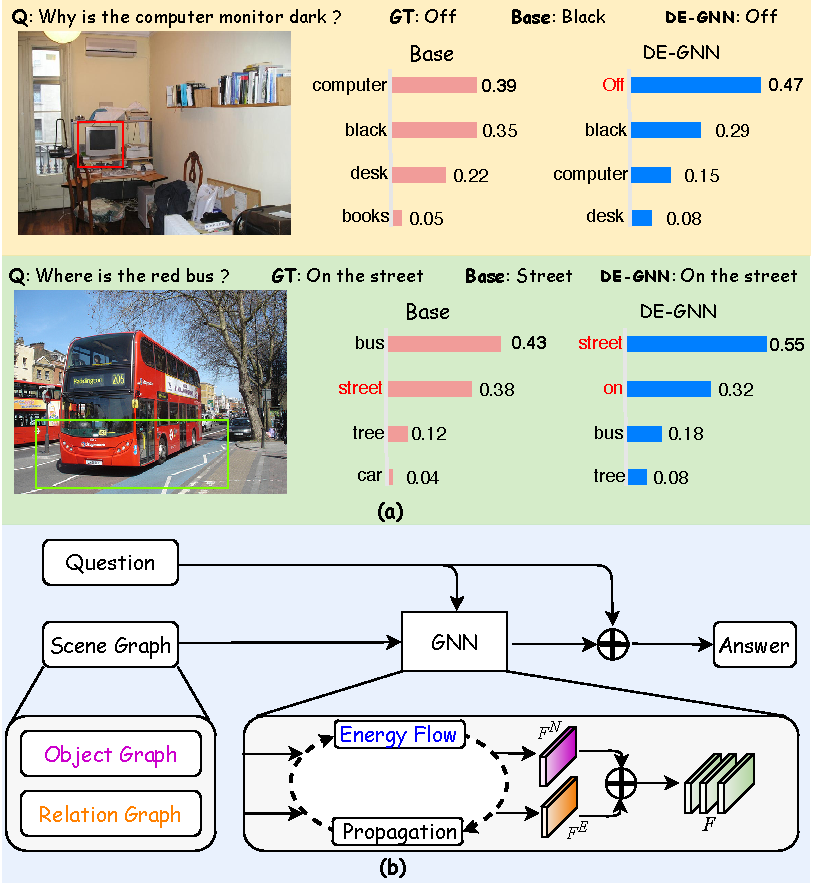
\includegraphics[scale=0.6]{./pic/intro5.pdf} 
    % \vspace{-0.1in}
    \caption{(a) Two key issues of traditional scene graph based models that we address: \textbf{false attribute selection} (bottom: select attribute ``black" instead of attribute ``off") and \textbf{missing relation} (top: missing ``on the") (b) Overview of our DE-GNN model. $F^N$ and $F^E$ are the node feature map and the relation feature map. $F$ is the full-scale feature map.} 
    \label{scene-graph} 
    \vspace{-0.1in}
\end{figure}

Visual Question Answering (VQA) tasks require a model to answer a free-form natural language question using visual information from an image. Scene graph (SG) reasoning is an essential instance of VQA tasks~\cite{DBLP:journals/corr/abs-2007-01072}. 
The model extracts objects' names, attributes, and relationships from the input images and organizes them into a graph representation to generate the scene graph.

SG representation modeling displays several virtues over classical techniques leveraging object features extracted from images since (a) the features in SG are presented in plain and free text form ~\cite{DBLP:journals/corr/abs-2101-05479} and (b) the graph structures of SG, which have better interpretability~\cite{DBLP:conf/bmvc/ZhangCX19}.
In this contribution, two reasoning methods on scene graphs are proposed. In particular, we: (i) consider scene graphs as probabilistic graphs and iteratively update nodes' probabilities using soft instructions extracted from questions such as Neural State Machine (NSM)~\cite{DBLP:conf/nips/HudsonM19,DBLP:conf/ijcnn/LeLV020}; (ii) apply Graph Neural Network (GNN) into scene graphs~\cite{inproceedings,DBLP:conf/iccv/LiGCL19} to learn a joint representation of the nodes and their relations, and then feed this representation into a predictor to generate the answer. 

Scene graph reasoning frameworks have proven to be useful in VQA tasks, e.g. \cite{johnson2015image,yang2020prior}. 
However, there still remains some imperfections. 

First, models tend to answer wrong for complex reasoning questions. 
Consider the ``why'' question in Fig.~\ref{scene-graph}(a) as an example, false attribute selection occurs because the model can not associate ``off'' relation with ``dark monitor'' object.
This is because attribute selections require supervision from objects, relations, and attributes, but existing methods fail at generating \emph{joint} representations for objects by using features from their neighbors \emph{and} their attributes. 
Generally, information from objects and relations connected to them are reconstructed into object features in GNN-based methods~\cite{xu2019spatial}. However, these encoding methods lack information from objects' attributes and neighbor objects. 
The NSM methods use attention mechanisms to update answer possibilities of objects, attributes, and relations, but they cannot learn the joint representation of all three types of information. 

Second, models answer poorly for questions that require information about the diverse relations and objects. For instance, for localization questions, as in the ``where'' type of questions, in Fig.~\ref{scene-graph}(a), we observe that relation missing occurs because the model can not capture the relation information ``on the''. This is because existing models have a strong bias towards node features, considering edge features as references. Generally in these models, nodes refer to objects, and edges refer to relations, which lead to the unbalance focus on objects and relations. 

% Empirically, we demonstrate that a correct relation representation is crucial to the VQA task and enables to alleviate the bottlenecks of VQA implied by inefficient usages of scene graph information described above.

Therefore, as a fix to the current ineffective strategies, we propose the Dual Energy-Flow Enhanced Graph Neural Network (DE-GNN) for VQA, introducing a novel scene graph reasoning model that extracts balanced feature maps from objects, attributes, and relations information in scene graphs. 
Concretely, as shown Fig.~\ref{scene-graph}(b), our DE-GNN model is composed of a scene graph generator, a question encoder, dual graph encoders, and a fusion module. 
Essentially, the scene graph generator extracts graphs out of the input images. 
Besides, to balance the importance of objects and relations, we transform scene graphs into a relation-significant modality, where nodes represent relations and edges represent objects, and an object-significant modality, in which nodes represent objects and edges represent relations. 
After receiving scene graphs in two modalities, dual graph encoders can produce feature maps focusing on both relations and objects.

Furthermore, to learn a node's joint representation from its attributes, edges, and adjacent nodes, we modify the gated graph neural network (GGNN) structure in our proposed DE-GNN by adding the energy-flow module. It is a bidirectional GRU that guides the internal information flow.
The encoder captures information from nodes, edges, and adjacent nodes that connect to them. 
As shown in Fig.~\ref{scene-graph}(b), the output feature map of the encoder passes through multi-head attention layers using question features extracted from the question encoder. 
Hence, the model dynamically focuses on the critical parts of the questions and uses the most similar part of the scene graph as the most adequate answer.

In summary, our main contributions are as follows:%\vspace{-0.05in}
\begin{itemize}
\setlength{\itemsep}{5pt}
\setlength{\parsep}{5pt}
\setlength{\parskip}{5pt}
\item We propose a novel DE-GNN model to learn a comprehensive and balanced representation of scene graphs by encoding graphs' object-significant modality and relation-significant modality.\vspace{-0.06in}

\item Our energy-flow module is suitable for processing graphs with meaningful edges and nodes with attributes.\vspace{-0.06in}

\item We conduct experiments on GQA and Visual Genome datasets and experimental results demonstrate that DE-GNN effectively improves the reasoning accuracy on semantically complicated questions.
% \item We show that our method outperforms other SG-based models in four scene graph datasets, which are generated from the VG dataset by four scene graph generation methods. Extensive experiments demonstrate the effectiveness of DE-GNN.
\end{itemize}\vspace{-0.06in}

\begin{figure*}[ht] 
    % \vspace{-0.5in}
    \centering 
    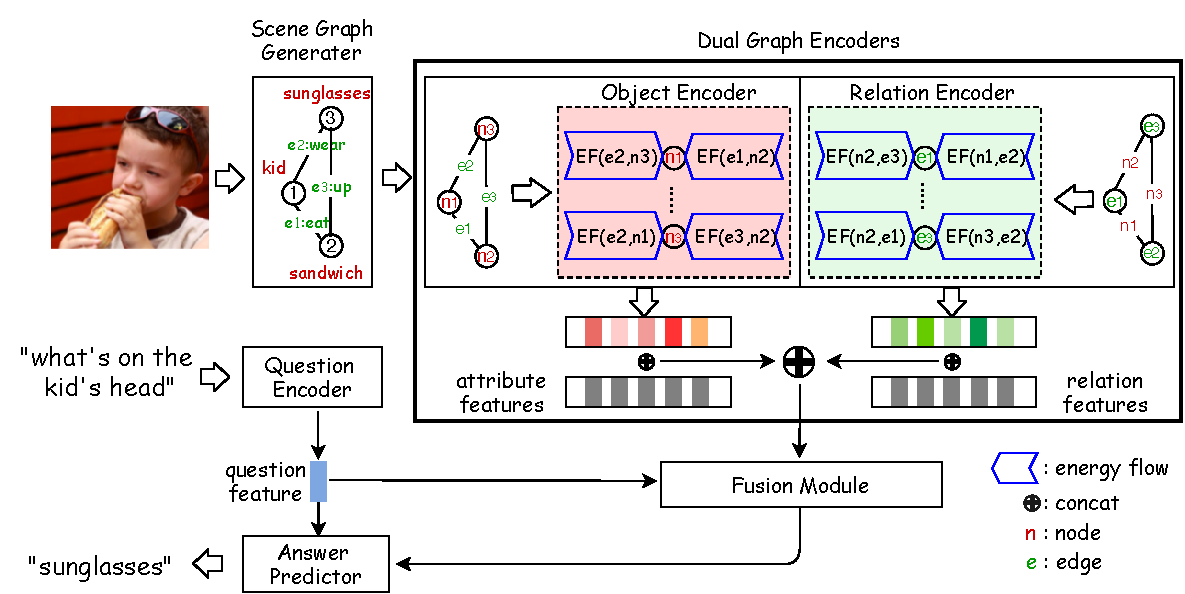
\includegraphics[width=1.0\textwidth]{./pic/DE-GNN.pdf} 
    % \vspace{-0.1in}
    \caption{Model structure of the Dual Energy-Flow enhanced Graph Neural Networks. EF stands for the energy-flow module. Images are transformed into scene graphs by the scene graph generator. The object-significant form and relation-significant form of the scene graph are injected into the object encoder and the relation encoder. Nodes' representations are generated from the sum of the energy-flow modules. The representations are then fused with question representations to predict answers.} 
    \label{fig2} 
    % \vspace{-0.2in}
\end{figure*}

\section{Related Work}
\noindent\textbf{Visual Question Answering.}
Most VQA approaches utilize a sequential model to encode the question and employ CNN-based pretrained models like Mask-RCNN or Faster-RCNN~\cite{DBLP:conf/cvpr/PatroN18,DBLP:conf/cvpr/NamHK17} to encode the image.
% Most VQA approaches utilize a question encoder architecture that can learn complex temporal dynamics using a sequence of hidden states. To encode the image, most VQA approaches employ CNN-based pretrained models like Mask-RCNN or Faster-RCNN~\cite{DBLP:conf/cvpr/FanZ18,DBLP:conf/cvpr/PatroN18,DBLP:conf/cvpr/NamHK17}. 
The image encoder and question encoder then pass through a multimodal fusion part and the output fusion vector pass through an answer predictor.
Many attention-based models~\cite{DBLP:conf/cvpr/00010BT0GZ18,DBLP:conf/cvpr/FanZ18,DBLP:conf/eccv/XuS16,DBLP:conf/nips/LuYBP16,DBLP:conf/iclr/HudsonM18} are proposed to model the relations between the images and the questions.
% To model the relations between the images and the questions, many attention-based models are proposed such as BUTD~\cite{DBLP:conf/cvpr/00010BT0GZ18}, SAT~\cite{DBLP:conf/cvpr/YangHGDS16}, question-guided spatial attention~\cite{DBLP:conf/eccv/XuS16}. In~\cite{DBLP:conf/nips/LuYBP16}, the authors proposed a hierarchical co-attention model that jointly implements both image-guided question attention and question-guided visual attention.  MacNet~\cite{DBLP:conf/iclr/HudsonM18} uses Mac-cells to combine attention and encoding function.
% However, there still exists a significant semantic gap between image and natural language. 
Transformer-based models such as Unicoder-VL~\cite{DBLP:conf/aaai/LiDFGJ20} can achieve outstanding performances on VQA tasks, yet these models are heavy to apply due to complicated pretraining strategies, extra datasets, time-consuming training, and hard to explain changeable environment. 
Instead, scene graph based models stands for an alternative that is more lightly and explainable.
% The pretraining tasks are time-consuming and hard to update under the changeable environment. 
% To solve the existing problems in attention-based and transformer-based VQA models, 
% We notice that scene graph is apply scene graphs as our reasoning model base.

\vspace{0.05in}
\noindent\textbf{Scene Graph Generation and Reasoning.}
Most scene graph generation (SGG) methods use object detection methods like mask-rcnn or faster-rcnn to extract region proposals from images~\cite{DBLP:conf/cvpr/XuZCF17,DBLP:conf/eccv/YangLLBP18,DBLP:conf/cvpr/ZellersYTC18,DBLP:conf/nips/WooKCK18,DBLP:conf/cvpr/DaiZL17,DBLP:conf/iccv/LiOZWW17,DBLP:conf/eccv/YinSLYWSL18,DBLP:conf/cvpr/TangNHSZ20}. 
% Methods to reduce the SGG training bias has been put forward~\cite{DBLP:conf/cvpr/TangNHSZ20}. 
% Due to the graph hierarchy extracted from images, 
Scene graph can promote explainable reasoning for downstream multimodal tasks such as VQA~\cite{DBLP:conf/bmvc/ZhangCX19}. 
In our work, scene graph generation methods are used to transform VQA datasets into scene graph datasets. 
Our model is tested on those generated datasets using various SGG methods.

In typical scene graph reasoning models, neural state machine~\cite{DBLP:conf/nips/HudsonM19} 
% first predicts a scene graph that represents its underlying semantics and 
% serves as a structured model of the world. 
% Then it 
performs sequential reasoning over the scene graph by iteratively traversing its nodes to answer a given question.
% or draw a new inference. 
% But, as we describe below, state machine-based models can not effectively capture complicated scene graph features.
% For instance, 
FSTT~\cite{inproceedings} uses GGNN based model to encode scene graphs.
% but it neglects vital information from edges and attributes. 
Relation-aware Graph Attention Network~\cite{DBLP:conf/iccv/LiGCL19} models multitype inter-object relations via a graph attention mechanism.
% to learn question-adaptive relation representations. 
However, the previous works are hard to fully utilize the attribute information and learn the comprehensive representation of scene graphs.
% using graph attention network. 
% Our model uses GGNN structure to learn more comprehensive scene graph representations. 

\vspace{0.05in}
\noindent\textbf{Graph Neural Network.}
% GNN~\cite{DBLP:journals/tnn/ScarselliGTHM09} are a class of traditional neural networks methods designed to infer on data described by graphs models. 
A group of graph neural networks (GNN) ~\cite{DBLP:journals/tnn/ScarselliGTHM09,DBLP:conf/cncl/WangGCL16,DBLP:conf/aaai/WangCGL18,DBLP:conf/aistats/SunL19,DBLP:conf/aaai/0001RFHLRG19,DBLP:conf/aaai/LiuCLZLSQ19} were proposed for different graph tasks.
% including graph representation learning. 
% Inspired by convolution neural network, 
Graph convolutional network (GCN)~\cite{DBLP:conf/iclr/KipfW17} improves GNNs efficiency with fast approximated spectral operations. 
GAT~\cite{DBLP:conf/iclr/VelickovicCCRLB18} introduces the attention mechanism to GNN, leveraging masked self-attentional layers to address the shortcomings of prior methods based on graph convolutions or their approximations. GGNN~\cite{DBLP:journals/corr/LiTBZ15} uses gated recurrent units (GRU) to accelerate the training speed and gain favorable inductive biases on large-scaled graphs.
% Similar to scene graphs, \cite{DBLP:conf/cncl/WangGCL16,DBLP:conf/aaai/WangCGL18,DBLP:conf/aistats/SunL19} apply GNN-based models on knowledge graphs.
% However, existing GNN-based models cannot effectively process graphs with node attributes and complicated labels.
Our DE-GNN model can learn a comprehensive representation using full-scale scene graph information from objects, attributes, and relations to overcome these problems.


\section{DE-GNN Methodology}

Beforehand, we define the VQA task. 
It is a classification task where for a given text question about an image, the goal is to output the correct answer. 
Formally, given question \emph{q} and image \emph{m}, the model aims to maximizing a conditional distribution over candidate answers \emph{a} as follows:
\begin{equation}\notag
    \hat{a} = \mathop{\arg\max}_{a \in A}p_\theta(a|q, m)
\end{equation}
where \emph{A} is the set of all possible answers, $p_\theta$ represents the VQA model with the trainable vector of parameters $\theta$ and $\hat{a}$ denotes the final answer.

Our proposed architecture designed for the VQA task is illustrated in Fig.~\ref{fig2}. 
Our model contains a scene graph generator, a question encoder, dual graph encoders and a fusion module. For the scene graph generator, we follow a codebase~\cite{tang2020sggcode} and other baselines referred in this work, which we will describe in the experiment section. 
For the question encoder, semantic questions are first projected into an embedding space using GLOVE pretrained word embedding model~\cite{pennington-etal-2014-glove}. 
After adding a positional encoding matrix into questions, we use long short-term memory (LSTM) networks to generate questions embedding $q \in R^{dim}$. 
We introduce our dual GGNN encoders in the following subsection.

\subsection{Object/Relation-Significant Graph}
We organize scene graphs into object-significant and relation-significant modalities. 

\medskip
\textbf{Object-Significant Graph.} We define the object significant modality as $\emph{G}_{obj}$, where every nodes represent objects in the image and every edges represent relations between two objects. Define $\emph{N}$ as the node set and $\emph{E}$ as the edge set. For $n_i, n_j \in \emph{N}$, $e_k \in \emph{E}$, $<n_i$ - $e_k$ - $n_j>$ denotes the relation tuple that represents the relation $e_k$ from object $n_i$ to object $n_j$. Note that relation tuples are not symmetrical: if $<n_i - e_k - n_j>$ is a valid relation tuple,  $<n_j - e_k - n_i>$ may not exist. Also, $n_i$ and $n_j$ may have several relations. 

\medskip
\textbf{Relation-Significant Graph.} We define relation significant modality as $\emph{G}_{rel}$, where every nodes represent relations between objects in the image and every edges represent objects, which is completely opposed to the object-significant modality. For $e_i, e_j \in \emph{E}$, $n_k \in \emph{N}$, $<e_i - n_k - e_j>$ denotes the relation tuple that represents the relations $e_i$ and $e_j$ have a shared object $n_k$. Note that relation tuples are also not symmetrical.

\begin{figure}[t] 
    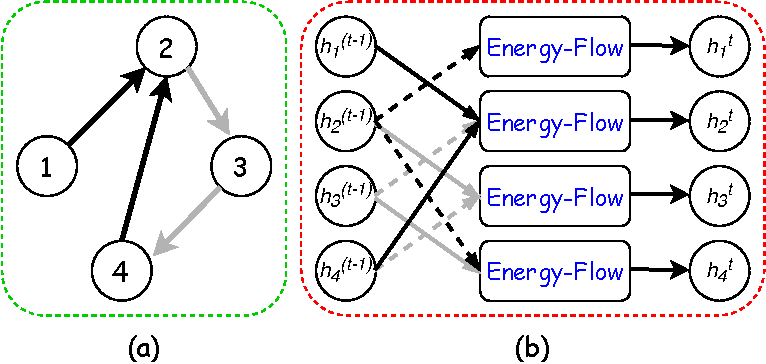
\includegraphics[width=1\textwidth]{./pic/EF.pdf} 
    \caption{Overview of the energy-flow module. (a) A graph example, where color denotes edge types. (b) Unrolled one timestep. Dotted lines are edges' backward representations.} 
    \label{EF} 
\end{figure}

\medskip
\textbf{Attribute types.} Define \emph{L} as attribute types (such as material, color, etc). 
For each node $n_i\in\emph{N}$ that corresponds to an object in the image, we define a set of $\emph{L}+1$ property variables ${\left\{ n_i^j\right\}}_{l=0}^L$, where $n_i^{0}$ represents $n_i$'s name embedding and $n_i^l$ represents the embedding of node $n_i$'s $l^{th}$ attribute (such as wooden, blue, etc).

\subsection{Dual Encoders}
We use two GGNN models as the encoders for object significant graphs and relation significant graphs. 
The GGNN for object graphs focuses on object features and the GGNN for relation graphs focuses on relation features. 
The dual encoder combination can balance the importance of relations and objects.
Prior to encoding, every input scene graph is transformed into an information tuple ($\emph{N}, \emph{E}, \emph{A}_{in}, \emph{A}_{out}$):\vspace{-0.02in}
\begin{itemize}
\setlength{\itemsep}{5pt}
\setlength{\parsep}{5pt}
\setlength{\parskip}{5pt}
    \item \emph{N} is a collection of node embeddings.\vspace{-0.06in}
    \item \emph{E} is a collection of directed edges that specify valid relation between nodes.\vspace{-0.06in}
    \item $\emph{A}_{in}$ is the adjacency matrix of incident edges.\vspace{-0.06in}
    \item $\emph{A}_{out}$ is the adjacency matrix of output edges.\vspace{-0.06in}
\end{itemize}

Let $h_i^t$ is the hidden state of node $n_i$ in GGNN at timestep $\emph{t}$, then at $\emph{t}=0$, we initialize $h_i^0$ as the GLOVE embedding of $n_i$ with appropriate zero padding:
\begin{equation}
    h_i^0 = [n_i^T, 0]^T  \, .
\end{equation}

The incident and output edges are retrieved in the respective adjacency matrices $\emph{A}_{in}$ and $\emph{A}_{out}$. 

\subsubsection{Energy-Flow Module}
To enhance the information transfer from edges and adjacent nodes to the updating nodes, we use the Energy-Flow module (EF) in Fig.~\ref{EF}.
EF module comes as a replacement of the fully-connected layers from the original GGNN model. 
% In the energy-flow module, consider, for instance the tuple, $<{n}_i, {e}_k, {n}_j>$ where the edge ${e}_k$'s embedding state $e_k$ and neighbor node ${n}_j$'s hidden state $h_j$ are injected into a bidirectional GRU network as input sequence while the node ${n}_i$'s hidden state $h_i$ is injected as GRU's initial hidden state. 
Consider a tuple $<{n}_i, {e}_k, {n}_j>$ as the processing sample of the energy-flow module. 
The embedding state, noted $\textit{e}_k$, of the edge ${e}_k$ and neighbor node ${n}_j$'s hidden state $\textit{h}_j$ are injected into a bidirectional GRU network as input sequence while the node ${n}_i$'s hidden state $\textit{h}_i$ is injected as the GRU's initial hidden state. 
The output of the GRU represents the updating information for hidden state $\textit{h}_i$, which corresponds to the key information from edge ${e}_k$ and node ${n}_j$ that is related to node ${n}_i$. 
The sum of every GRU output is ${n}_i$'s total information gain from ${n}_i$'s adjacent nodes and edges. 
We detail the complete energy-flow module formula as follows:
\begin{gather}\notag
    EF_i(A_{in}) = \sum\limits_{k,j}^{<n_i,e_k,n_j>\in A_{in}} \text{GRU}([\textit{e}_k, \textit{h}_j], \textit{h}_i) \, , \\ \notag
    EF_i(A_{out}) = \sum\limits_{k,j}^{<{n}_j,{e}_k,{n}_i>\in A_{out}} \text{GRU}([\textit{e}_k, \textit{h}_j], \textit{h}_i) \, ,\notag
\end{gather}
where $EF_i(A_{in})$ is ${n}_i$'s incident information gain, and $EF_i(A_{out})$ is ${n}_i$'s output information gain.



\subsubsection{Propagation Model}

At timestep $t$, the hidden states of all nodes are updated by the following gated propagator module:
\begin{gather}\notag
    k_{i}^t = [EF_i^t(A_{in}), EF_i^t(A_{out})] \, ,
\end{gather}
where $k_{i}^t$ is the node ${n}_i$'s representation from all its incident edges, output edges and adjacent nodes.

% The remaining are 
Then, we adopt GRU-like updates to incorporate information from adjacent nodes and from the previous timestep leading to an update of each node's hidden state:
\begin{gather}\notag
    % c_i^t = W_i^T[h_i^{(t-1) T}, k_{i}^{(t-1) T}]^T + b\\
    c_i^t = [h_i^{(t-1)}, k_{i}^{(t-1)}] W + b \, ,\\\notag
    z_i^t = \sigma(U^z c_i^t) \, , \\\notag
    r_i^t = \sigma(U^r c_i^t)\, , \notag
\end{gather}
where $W, U^z$ and $U^r$ are referred to as the trainable weight matrices and $b$ as a bias term.
At timestep $t$, we denote by $z_i^t$ and $r_i^t$ the update and reset gates, respectively. Then we have:
\begin{gather}\notag
    \tilde{h}_i^t = \text{tanh}(U_1 k_{i}^{(t-1)} + U_2(r_u^t \odot h_i^{(t-1)})) \, ,\\\notag
    h_i^t = (1-z_i^t)\odot h_i^{(t-1)} + z_i^t\odot \tilde{h}_i^t \, .\notag
\end{gather}
Here, $U_1$ and $U_2$ denote the trainable parameters of the linear layers, the operator $\odot$ is the element-wise multiplication.
% and $h_i^t$ designates the updated hidden state for node ${n}_i$. 
After $T$ steps, the GGNN encoder generates the final hidden state map $G$ of the graph. 
Finally, we compute the graph embedding $g_i \in G$ for node ${n}_i$ as follows:
\begin{equation}\notag
    g_i = \sigma( \emph{f}(h_i^T, n_i)) \, ,
\end{equation}
where $\emph{f}(\cdot, n_i)$ is the multi-layer perceptron (MLP) which receives the concatenation of $h_i^T$ and $n_i$, then generates the final representation of node ${n}_i$. 

\subsection{Fusion Module and Answer Predictor}

Once the dual encoders, embedded in our model, output the node and relation features, we first fuse the attributes into feature maps. 
For node feature map $G^N$ and relation feature map $G^E$, the fusion feature map $F^N$ and $F^E$ are defined as

{\small \begin{equation}\notag
F_i^N= \begin{cases}
[g_i^N, n_i^0]  \\
\cdots, \\
[g_i^N, n_i^L]
\end{cases} 
,\, F_j^E = [g_j^E, e_j] , \,
    F = [F^N, F^E]  ,
\end{equation}
}

where $F_i^N$ indicates the fusion features of node $i$ and $g_i^N$ is node $i$'s representation from the GGNN encoder. 
We denote by the vector $(n_i^0, \cdots,n_i^L)$ the embeddings attributes of node $i$. 
$F_j^E$ corresponds to the fusion feature of edge $j$. $g_j^E$ is edge $j$'s representation from the GGNN encoder. 
$e_j$ is $j$-th edge original embedding. 
The full-scale feature map, noted $F$, is obtained by concatenating $F^N$ and $F^E$.

Then, the question embedding $\emph{q}$ generated from the LSTM encoder and the full-scale feature map $F$ are fed into a multi-head attention layer, where the query is stored in $F$ and the key and values are stored in $\emph{q}$.
% Scores for every features are calculated. 
The reasoning vector, noted $\emph{r}$, and which stems from the graph and the question, is computed using a weighted sum of the feature map using the scores output from the attention layer, i.e.,
\begin{gather}\notag
    r = \text{Attention}(F, q) \, . 
\end{gather}

Regarding the answer predictor module, we adopt a two-layer MLP noted by $f(\cdot)$. 
This MLP can be viewed as a classifier over the set of candidate answers. 
The input of the answer predictor is the concatenation vector $(\emph{q},\emph{r})$. 
Such a classifier has been applied in many VQA models as in NSM~\cite{DBLP:conf/nips/HudsonM19} and MacNet~\cite{DBLP:conf/nips/LuYBP16}.
Formally, the output answer reads:
\begin{gather}\notag
    \hat{a} = \mathop{\arg\max}(\text{softmax}(f((\emph{q},\emph{r}))))\, .
\end{gather}

We provide in the next section, various numerical experiments to validate our newly introduced model.


\section{Experiments}\label{sec:experiments}

\subsection{Datasets}

-- The \textbf{Visual Genome} dataset contains $108 \, 077$ images with comprehensively annotated objects, attributes, and relations. To enrich the scene graph annotation in Visual Genome, we use a scene graph generation method and motifs~\cite{DBLP:conf/cvpr/ZellersYTC18} to generate a new scene graph dataset called \textbf{motif-VG}. 
Compared with the Visual Genome dataset, motif-VG has the same images and questions-answers tuples, but has scene graph annotations with different qualities and biases. 
We split both datasets into train, valid, and test sets using a $7:1:2$ ratio. 

\noindent --  The \textbf{GQA} dataset~\cite{DBLP:conf/cvpr/HudsonM19} focuses on real-world reasoning, scene understanding and compositional question answering. 
It is composed of 113k images and 22M questions of assorted types and varying compositionality degrees, measuring performance on an array of reasoning skills such as object and attribute recognition, transitive relation tracking, spatial reasoning, logical inference and comparisons.



\subsection{Implementation Details}
We use the 50-dimensional GLOVE word embeddings model ~\cite{pennington-etal-2014-glove} to project words and questions embeddings into the scene graph. 
In order to record the questions' position information, we set up the positional encoding matrix $\textrm{PE}$ as follows:
\begin{gather}\notag
    \textrm{PE}_{\texttt{pos}=2\emph{i}} = \sin(\texttt{pos}/10000^{2i/d_{\textrm{m}}}) \, ,\\
    \textrm{PE}_{\texttt{pos}=2\emph{i}+1} = \cos(\texttt{pos}/10000^{2i/d_{\textrm{m}}}) \, , \notag
\end{gather}
where $\texttt{pos}$ is the position of the word in the question sequence.
% If $\texttt{pos}$ is odd, the position information is generated by a $\sin$ function, else, it is generated by a $\cos$ function. 
% We also let model dimension equal to $d_{\textrm{m}}=50$.
% After adding position information, 
The question embeddings are injected into a single-directional GRU network. The dimension of the hidden layers of the GRU is 100, and the dropout rate is 0.2.

% In our energy-flow enhanced GGNN encoder, the propagator time step is 5. 
In the GGNN encoder, the propagator time step is 5. 
% , and we use a bidirectional GRU as our energy-flow module. 
We set the dimension of energy-flow's GRU hidden layer to 50. 

In the fusion module, we apply a multi-head attention layer with 5 heads and no dropout. Regarding the answer predictor, we select the top-2000 answer candidates and use a 2-layer MLP as the output classifier.

We use Adam~\cite{DBLP:journals/corr/KingmaB14} as the optimizer, and Cross Entropy Loss as the loss function during the training of our model. 
More details are presented in supplementary materials.
% For motif-VG dataset, we set the batch size to 512. For Visual Genome ground truth dataset and GQA dataset, we set the batch size to 16 due to their abundant scene graph annotations.

% The learning rate is decaying with respect to the epoch number. 
% We initialize the learning rate to be $1e^{-3}$, and when 30\% epochs finish, the learning rate drops to $2e^{-4}$. When 60\% epochs finish, the learning rate drops to $4e^{-5}$ and it becomes $8e^{-6}$ after 80\% epochs finish. We train our model and other baselines on a single V100 GPU.

% \begin{figure}[h] 
% \mbox{ \hspace{-0.12in}
%     \includegraphics[width=1.6in]{fig/fig5-left.eps} \hspace{-0.12in}
%     \includegraphics[width=1.6in]{fig/fig5-right.eps} 
% }
%     \caption{The validation accuracy curves for ablation experiments} 
%     \label{ablation-figure} 
% \end{figure}
\begin{table*}[ht]
\centering
    \begin{tabular}{l|lllllllll}
    \hline
    \textbf{Question type}&\textbf{What}&\textbf{Color}&\textbf{Where}&\textbf{How}&\textbf{Who}&\textbf{When}&\textbf{Why}&\textbf{Overall}\\
    \hline
     Percentage &(54\%) &(14\%) &(17\%) &(3\%) &(5\%) &(4\%) &(3\%) &(100\%)\\
    \hline
    \multicolumn{9}{c}{\bf VG-GroundTruth} \cr\hline %& & & &\makecell[c]{\textbf{VG-GT}}& & & &\\
    % \hline
     NSM~\cite{DBLP:conf/nips/HudsonM19} &33.1 &52.4 &51.0 &52.9 &49.8 &77.9 &12.3 &45.1\\
     MLP~\cite{DBLP:conf/eccv/JabriJM16} &- &- &- &- &- &- &- &58.5\\
     F-GN~\cite{DBLP:conf/bmvc/ZhangCX19}&60.9 &53.6 &62.0 &46.2 &63.3 &\textbf{83.7} &50.9 &60.1\\
     U-GN~\cite{DBLP:conf/bmvc/ZhangCX19}&61.6 &54.0 &62.4 &45.9 &63.9 & 83.2 &50.3 &60.5\\
     SAN~\cite{DBLP:conf/cvpr/FanZ18} &- &- &- &- &- &- &- &62.6\\
     FSTT~\cite{inproceedings} &65.5 &45.6 &70.1 &47.8 &68.3 &82.1 &91.5 &65.6\\
     ReGAT~\cite{DBLP:conf/iccv/LiGCL19} &72.1 &\textbf{70.8} &64.4 &\textbf{68.9} &72.7 &65.0 &92.3 &71.2\\
     DE-GNN (ours) &\textbf{75.9} &64.9 &\textbf{73.1} &66.8 &\textbf{82.6} &81.4 &\textbf{98.8} &\textbf{75.4}\\
    \hline
     \multicolumn{9}{c}{\bf Motif-VG} \cr\hline
    % \hline
     NSM~\cite{DBLP:conf/nips/HudsonM19} &31.8 &62.4 &53.1 &51.4 &47.6 &83.3 &10.9 &43.1\\
     FSTT~\cite{inproceedings} &48.8 &40.4 &49.2 &40.1 &40.6 &54.5 &70.3 &48.1\\
     F-GN~\cite{DBLP:conf/bmvc/ZhangCX19} &58.7 &60.8 &60.4 &47.2 &61.8 &84.8 &49.0 &60.0\\
     U-GNN~\cite{DBLP:conf/bmvc/ZhangCX19} &59.4 &58.2 &60.3 &54.3 &66.6 &\textbf{85.3} &48.1 &60.5\\
     ReGATT~\cite{DBLP:conf/iccv/LiGCL19} &75.4 &\textbf{69.2} &57.6 &\textbf{69.9} &69.1 &57.4 &91.8 &69.9\\
     DE-GNN (ours) &\textbf{79.4} &67.6 &\textbf{62.7} &65.3 &\textbf{72.8} &63.0 &\textbf{96.1} &\textbf{72.9}\\
    \hline
    \end{tabular}
\caption{\label{VG-detail}
Performance on different question types of VG dataset.}
\end{table*}

\begin{table*}[htbp]
    \begin{floatrow}
    \capbtabbox{
     \begin{tabular}{lll}
      \hline
      \textbf{Models}&\textbf{Acc.}\\
      \hline
      \textbf{Base} & 35.4\% \\
      \hline
       +\emph{EF} & \emph{unstable} \\
       +\emph{Obj} & 35.4\% \\
       +\emph{Obj}+\emph{EF}& 39.3\% \\
       +\emph{Rel} & 35.2\% \\
       +\emph{Rel}+\emph{EF}& 38.8\% \\
       +\emph{Obj}+\emph{Rel} &\textbf{67.9}\%\\
      \hline
       + (w/o \emph{QF}) & 54.9\% \\
       + (w/o \emph{attr}) & 71.6\% \\
       + (w/o \emph{rela}) & \textbf{74.5}\% \\
      \hline
       DE-GNN(ours) & \textbf{75.2}\%\\
      \hline
    \end{tabular}
    }{
     \caption{Ablation study}
     \label{ablation-study}
    }
    \capbtabbox{
     %\rowcolors{1}{blue!10}{white}
     \begin{tabular}{llllll}
       \hline
       \textbf{Models}&\textbf{Binary$\uparrow$}&\textbf{Open$\uparrow$}&\textbf{Validity$\uparrow$}&\textbf{Distribution$\downarrow$}&\textbf{Accuracy$\uparrow$}\\
    \hline
     Human &91.20 &87.40 &98.90 &- &89.30\\
     BottomUp &66.64 &34.83 &96.18 &5.98 &49.74\\
     MAC &71.23 &38.91 &96.16 &5.34 &54.06\\
     SK T-Brain &77.42 &43.10 &96.26 &7.54 &59.19\\
     PVR &77.69 &43.01 &\textbf{96.45} &5.80 &59.27\\
     GRN &77.53 &43.35 &96.18 &6.06 &59.37\\
     Dream &77.84 &43.72 &96.38 &8.40 &59.72\\
     LXRT &77.76 &44.97 &96.30 &8.31 &60.34\\
     NSM &78.94 &49.25 &96.41 &\textbf{3.71} &63.17\\
     ReGAT &\textbf{83.57} &62.58 &92.70 &9.32 &70.50\\
     DE-GNN(ours) &69.79 &\textbf{72.21} &93.80 &3.78 &\textbf{71.21}\\
    \hline
    \hiderowcolors
    \end{tabular}
    }{
     \caption{Performance on the GQA dataset.}
     \label{GQA}
    }
    \end{floatrow}
\end{table*}

\subsection{Empirical Results}
In this subsection, we provide the experimental results on various datasets mentioned above. 
The different baselines compared in our experiments all use various methods to generate the scene graphs for images. 
In order to ensure general fairness across the methods, we implement them from scratch, removing their scene graph generation parts to eliminate the interference of different generation methods.

\subsubsection{Results on VG dataset} Table~\ref{VG-detail} reports the results on the test sets of the VG ground truth datasets and the motif-VG dataset. Compared to the baseline models, we can observe that our DE-GNN model outperforms the others at $\textbf{3\%}$-$\textbf{4\%}$. In addition, we provide detailed results on the VG dataset and motif-VG dataset with different question types. Compared to the other scene graph based VQA models, our model performs well in ``what", ``where", ``who" and ``why" types. Specially, our model has $\textbf{6\%}$ accuracy improvement in ``\textbf{why}" type questions, which highly requires VQA models' ability to jointly exploit objects, relations and attributes. However, our model's comprehensive representations influence the accuracy on simple questions. In ``color'' type, our model achieves 2nd score.

% In addition, the stability of our model is conspicuous. Our model can achieve consistent and stable performance under different scene graph qualities. Our model's performances under four different scene graph datasets only suffer 3\% fluctuation,
% while FSTT suffers from a 4.7\% fluctuation and Re-GAT suffers from a 26.9\% fluctuation. 
% Figure~\ref{four-graph} is the intuitive validation curves on four datasets. Our model in the blue line can steadily converge at nearly 15 epochs under four different datasets with various scene graph qualities. 

\begin{table}
    \begin{tabular}{llll|l}
    \hline
     \textbf{Models} & FSTT & ReGAT & DE-GNN & Case Number \\
    \hline
     Relation & 45.9\% & 44.6\% & \textbf{32.9}\% & 7913\\
     Object &58.6\% & 47.3\% & \textbf{25.2}\% & 4414\\
     Attribute & 49.6\% & 22.8\% & \textbf{16.8}\% & 15483\\
    \hline
    \end{tabular}
\caption{\label{badcase}
Error rate analysis on motif-VG dataset. 
}
\end{table} 

\subsubsection{Results on GQA dataset} We report in Table~\ref{GQA} the detailed results on the test sets of the GQA dataset. Compared to the baseline models, our DE-GNN model achieves state-of-the-art accuracy performance. We also evaluate our model and other baselines across GQA dataset's various metrics, where "Binary" represents binary-answer questions, "Open" stands for open domain questions and "Distribution" corresponds to the distance between prediction distribution and standard answer distribution. In open domain questions which are difficult for reasoning, our model outperforms the others at $\textbf{10\%}$. In distribution metric, our model also achieves 2nd score compared to other baselines. However, the comprehensive representation may interfere with DE-GNN's judgment of simple problems such as ``Binary'' questions.

\subsubsection{Error Rate Analysis} To demonstrate that our dual encoders structure can intensify the model's perception of relation features and learn a comprehensive representation from nodes, attributes, and relations information, we establish an error rate analysis for baselines and DE-GNN on motif-VG.

The badcases are classified into object, relation and attribute. We present Table~\ref{badcase} the results for our error rate analysis. Our DE-GNN model surpasses all baselines in the terms of objects detection and our model does well in relation retrieval, outperforming GNN based FSTT and Re-GAT. This proves our model does alleviate the unbalance focus on objects and relations.
Also, our model reduces nearly half of the wrong answers in FSTT, Re-GAT in the attribute aspect, which greatly improves the false attribute selection phenomenon.

% The question fusion module, which concatenates the question vector with the reasoning vector before entering into the answer predictor module, is a common module in VQA models, including NSM, FSTT, and our DE-GNN model. This method has been shown to improve the accuracy of VQA models. However, from a cognitive point of view, the question fusion module lacks of interpretability since the question features are included in the reasoning vector of the model. 
% Also, the addition of the question fusion module may lead the reasoning model to only \emph{guess answers} from questions, which negatively influences the reasoning itself. 
% We retrain our model and other baselines without the question fusion module to evaluate the reasoning ability without the influence of outer question information. 
% Table~\ref{model-without-fusion} shows the results of models without question fusion module. 
% Note that there is no question fusion module in the Re-GAT baseline, so the Re-GAT result is the same as Table~\ref{citation-guide}.
% After reducing the concatenation of the question vector and reasoning vector, FSTT, NSM, and our DE-GNN model suffer accuracy recessions. Without question fusion, our model still outperforms other baselines.

\begin{figure*}[ht] 
    \vspace{-0.5in}
    \centering 
    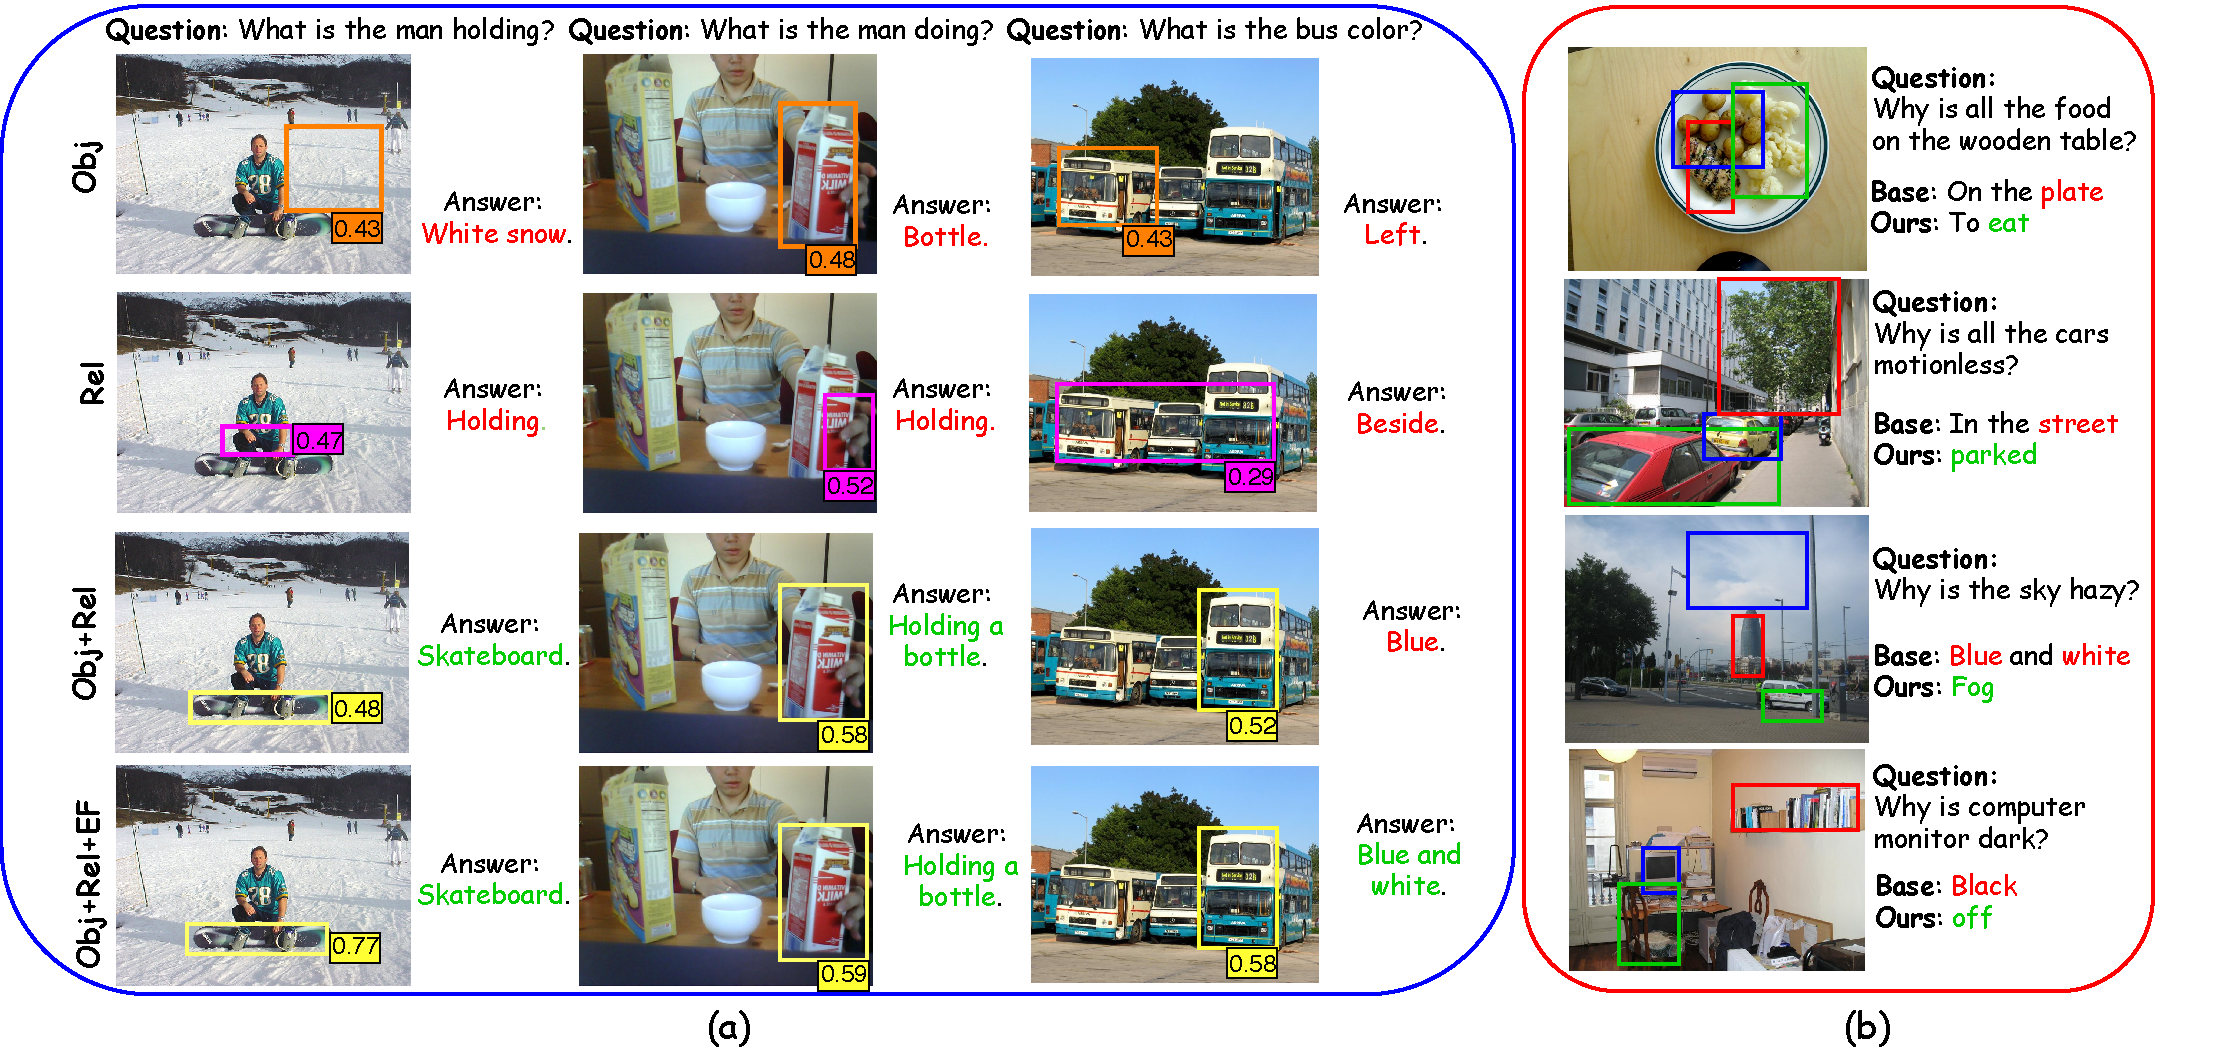
\includegraphics[width=1\textwidth]{./pic/visual_aaai2.pdf} 
    % \vspace{-0.1in}
    \caption{Examples of generated answers and top attention scores. Answers in red means wrong and answers in green means right. The left plot and right plot show the visualization of ``what" and ``why" question types. From the left plot (a), we observe that our approach can correctly select answer from objects, relations and attributes. From the right plot (b), we note that our model can handle comprehensive reasoning questions.} 
    \label{visual} 
    \vspace{-0.1in}
\end{figure*}

\begin{figure*}[ht] 
    \centering 
    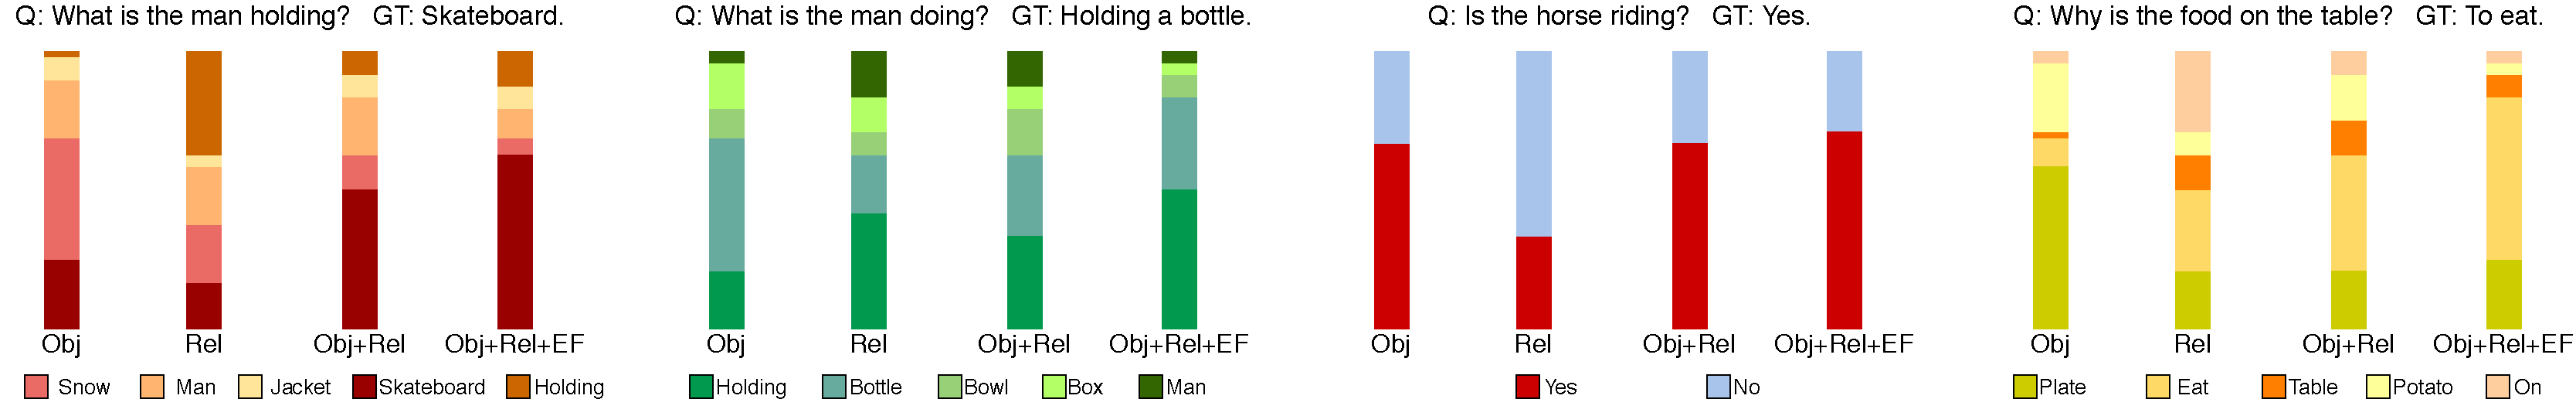
\includegraphics[width=1\textwidth]{./pic/visual_detail.pdf} 
    % \vspace{-0.1in}
    \caption{Examples of top 5 attention scores of candidate answers for different types of questions.} 
    \label{visualbis} 
\end{figure*}


\subsection{Ablation Study}
We compare several ablated forms of DE-GNN with our complete one. 
The accuracy results for each variant of DE-GNN are reported in Table~\ref{ablation-study}. 
We use the original GGNN network as the \emph{base} model to encode scene graphs.
In Table~\ref{ablation-study}, the \emph{Obj} model represents the original GGNN network processing \emph{object-significant} graphs. The \emph{Rel} model represents the original GGNN network processing \emph{relation-significant} graphs.
The \emph{Obj-EF} model corresponds to the object encoder part of our DE-GNN model, which contains one energy-flow enhanced GGNN network to encode \emph{object-significant} graphs. 
The \emph{Rel-EF} model is the other half of our DE-GNN model, which contains one energy-flow enhanced GGNN network to encode \emph{relation-significant} graphs.

\subsubsection{Effect of dual encoder structure} We first validate the efficacy of applying dual structure to balance the importance of relations and objects by splitting our DE-GNN into an object-single model (noted \emph{Obj}) and a relation-single model (noted \emph{Rel}). Table~\ref{ablation-study} shows that both \emph{Obj} and \emph{Rel} models perform poorly, at about 35.3\%. 
It also shows that both relations and objects are vital to VQA performance. 
Absence of any of those modules leads to severe accuracy recession. 
Combining the object-single model and the relation-single model leads to an empirical gain of approximately 35\% accuracy upward, which shows that the dual structure is significant in balancing relation and object information. 

\subsubsection{Effect of the energy-flow module} We corroborate the effectiveness of applying energy-flow structure to learn a more comprehensive representation for scene graphs than the original GGNN structure, which represents the baseline in Table~\ref{ablation-study}. 
We compare the \emph{Obj+EF} model and the \emph{Obj} model, which both learn representations from object-significant graphs, and note that after adding the energy-flow structure, there is an accuracy improvement of 3.9\%. 
We also compare the \emph{Rel+EF} model and the \emph{Rel} model and observe an accuracy improvement of 3.6\%. 
The \emph{Obj+Rel} model is DE-GNN without energy-flow module. 
Comparing with DE-GNN, there is a 7.3\% accuracy improvement after adding the energy-flow module. 
These empirical results show that energy-flow structure can successfully improve the representation quality of scene graphs. 

\subsubsection{Effect of explicit modeling} To demonstrate the impact of the explicit modeling of attributes and relations in DE-GNN, the \emph{w/o attr} model removes the explicit attribute modeling part from DE-GNN and the \emph{w/o rela} model removes the explicit relation modeling part. 
Removing attribute modeling leads to a drop of 3.6\% in accuracy, while the relation modeling has only a 0.7\% accuracy positive influence.


% To better understand how our dual energy-flow enhanced GNN model inferences and answers questions, we further visualize and compare the attention maps learned by the ablated models in the following subsection.

\subsection{Visualization}
To illustrate the effectiveness of the dual encoder structure and the energy-flow module in our DE-GNN model, we compare the top attention score learned by DE-GNN model with the scores learned by our \emph{Obj}, \emph{Rel} and \emph{Obj+Rel} models. 
Fig.~\ref{visual} provides a visualization of our results.

The left blue plot shows the visualization on "what" question type. 
Examples on all three columns of Fig.~\ref{visual} correspond to "what" type of questions aimed at retrieving either node, relation or attribute information. 
Comparing row 1, row 2 with row 3, \emph{Obj} and \emph{Rel} models have strong attention bias toward objects and relations, while their combination, i.e. \emph{Obj+Rel}, balances the attention on both sides and captures correct answers. 
Comparing row 3 with row 4, the addition of the energy-flow module increases the attention score of correct answers. 

The right red plot shows the visualization on ``why'' type of question. 
For ``why'' questions, models jointly exploit objects, relations and attributes to generate answers. 
Using dual encoder structures ans the energy-flow module, our DE-GNN can generate correct answers and achieves \textbf{96.1\%} accuracy on ``why" questions.

Fig.~\ref{visualbis} exhibits the details of top 5 attention scores for different types of questions. 
Our dual encoder structures and energy-flow module significantly increase the attention scores of correct answers.


\section{Conclusion}
In this work, 
% we study classical scene graph reasoning methods such as GNN-based models and Neural State Machine for Visual Question Answering tasks. 
% We observe that neither can existing models \emph{jointly} exploit objects, relations, and attributes in SG, nor can they balance the importance of objects and relations.
% To address this problem, 
we propose the DE-GNN model, which encodes each scene graph into feature representations via an object encoder and a relation encoder generating full-scale feature maps using nodes, attributes, and relations information and demonstrate our model can effectively boost performances on various datasets. 
% We demonstrate the effectiveness of our method on the various datasets achieving significant improvement and state-of-the-art results. 
Ultimately, we will dynamically adjust the model according to difficulty of the question, and improve our model's accuracy on simple questions.


\newpage

% Use \bibliography{yourbibfile} instead or the References section will not appear in your paper
% \nobibliography{custom}

\clearpage
\bibliography{custom}


\end{document}
